%%%%%%%%%%%%%%%%%%%%%%%%%%%%%%%%%%%%%%%%%
% Short Sectioned Assignment
% LaTeX Template
% Version 1.0 (5/5/12)
%
% This template has been downloaded from:
% http://www.LaTeXTemplates.com
%
% Original author:
% Frits Wenneker (http://www.howtotex.com)
%
% License:
% CC BY-NC-SA 3.0 (http://creativecommons.org/licenses/by-nc-sa/3.0/)
%
%%%%%%%%%%%%%%%%%%%%%%%%%%%%%%%%%%%%%%%%%

%----------------------------------------------------------------------------------------
%	PACKAGES AND OTHER DOCUMENT CONFIGURATIONS
%----------------------------------------------------------------------------------------

\documentclass[paper=a4, fontsize=11pt]{scrartcl} % A4 paper and 11pt font size

\usepackage{listings}
\usepackage[utf8]{inputenc}
\usepackage[T1]{fontenc} % Use 8-bit encoding that has 256 glyphs
\usepackage{lmodern}
\usepackage{fourier} % Use the Adobe Utopia font for the document - comment this line to return to the LaTeX default
\usepackage[english]{babel} % English language/hyphenation
\usepackage{amsmath,amsfonts,amsthm} % Math packages

\usepackage{graphicx}

\usepackage{float}

\usepackage{lipsum} % Used for inserting dummy 'Lorem ipsum' text into the template

\usepackage{sectsty} % Allows customizing section commands
\allsectionsfont{\centering \normalfont\scshape} % Make all sections centered, the default font and small caps

\usepackage{fancyhdr} % Custom headers and footers
\pagestyle{fancyplain} % Makes all pages in the document conform to the custom headers and footers
\fancyhead{} % No page header - if you want one, create it in the same way as the footers below
\fancyfoot[L]{} % Empty left footer
\fancyfoot[C]{} % Empty center footer
\fancyfoot[R]{\thepage} % Page numbering for right footer
\renewcommand{\headrulewidth}{0pt} % Remove header underlines
\renewcommand{\footrulewidth}{0pt} % Remove footer underlines
\setlength{\headheight}{13.6pt} % Customize the height of the header

\numberwithin{equation}{section} % Number equations within sections (i.e. 1.1, 1.2, 2.1, 2.2 instead of 1, 2, 3, 4)
\numberwithin{figure}{section} % Number figures within sections (i.e. 1.1, 1.2, 2.1, 2.2 instead of 1, 2, 3, 4)
\numberwithin{table}{section} % Number tables within sections (i.e. 1.1, 1.2, 2.1, 2.2 instead of 1, 2, 3, 4)

\setlength\parindent{0pt} % Removes all indentation from paragraphs - comment this line for an assignment with lots of text




%----------------------------------------------------------------------------------------
%	TITLE SECTION
%----------------------------------------------------------------------------------------

\newcommand{\horrule}[1]{\rule{\linewidth}{#1}} % Create horizontal rule command with 1 argument of height

\title{	
\normalfont \normalsize 
\textsc{FGV - Fundação Getúlio Vargas} \\ [25pt] % Your university, school and/or department name(s)
\horrule{0.5pt} \\[0.4cm] % Thin top horizontal rule
\huge Trabalho Final - Wealth Management \\ % The assignment title
\horrule{2pt} \\[0.5cm] % Thick bottom horizontal rule
}

\author{Pedro Montero Mattos} % Your name

\date{\normalsize September 29, 2016} % Today's date or a custom date

\begin{document}

\maketitle % Print the title

%----------------------------------------------------------------------------------------
%	PROBLEM 1
%----------------------------------------------------------------------------------------

\section{Introduction}

We aim to study different rebalance techniques and their performances. It is of interest of every wealth or asset manager to use a portfolio rebalance technique that allows their funds to both perform and hedge from drawdowns.

Using real Brazilian data we simulated the performance of three strategies known as: Equally weighted portfolio, Minimum Variance Portfolio and Tangency Portfolio (Or maximum Sharpe Portfolio).

We tested those strategies for three different rebalancing frequencies: Monthly, Quarterly and Annual.

First we wanted to find which rebalance frequency works best. The data provided weak evidence that lower frequencies, i.e. Annual and Quarterly, are usually more effective, but it varies a little depending on the strategy.

Secondly, we wanted to find which strategy works best, despite its rebalancing frequency. The data provided consistent evidence that for our sample the Tangency portfolio outperforms the Minimum Variance Portfolio, which outperforms the Equally Weighted Portfolio.

To check our conclusions for robustness we used Monte Carlo Simulation on our sample to generate alternative scenarios. Since rebalancing techniques are specially useful when they protect the portfolio against drawdowns we chose the 1\% and 5\% worst scenarios to backtest the strategies.

The new experiment provided evidence that defies our previous conclusion that lower frequency rebalancing is more effective than high frequency rebalancing but reassured our conclusion that the Tangency portfolio is the most effective strategy.


\section{Strategies}

\subsection{Equally Weighted Portfolio}

This very simple strategy consists on assigning equal shares of the portfolio's assets to every asset class.
Thus each asset class will have a relative weight of:

$$w_i = \frac{1}{n}$$

Where $n$ is the number of asset classes available. In our particular case, 3.

\subsection{Minimum Variance Portfolio}

When we construct a Efficient Frontier following \textit{Markowitz (1952)} the Minimum Variance Portfolio is the left-most point in the frontier, which is the efficient portfolio with least variance of all.

\subsection{Tangency Portfolio}

On the same abovementioned frontier, the Tangency portfolio is the one which the return / variance ratio is the maximum. That is, the Sharpe Index has its maximum value among the frontier portfolios.


\section{Assets}

Initially we intended to use IBOV, IMA-S, and IMA-B in our experiment. But because the IMA-S has basically no volatility, both the frontier strategies tended to allocate 100\% on it, causing that experiments to be inconclusive. So, despite the professors's recommendation,  we decided to switch IMA-S for the local currency against American dollars (USDBRL).

\begin{figure}[H]
  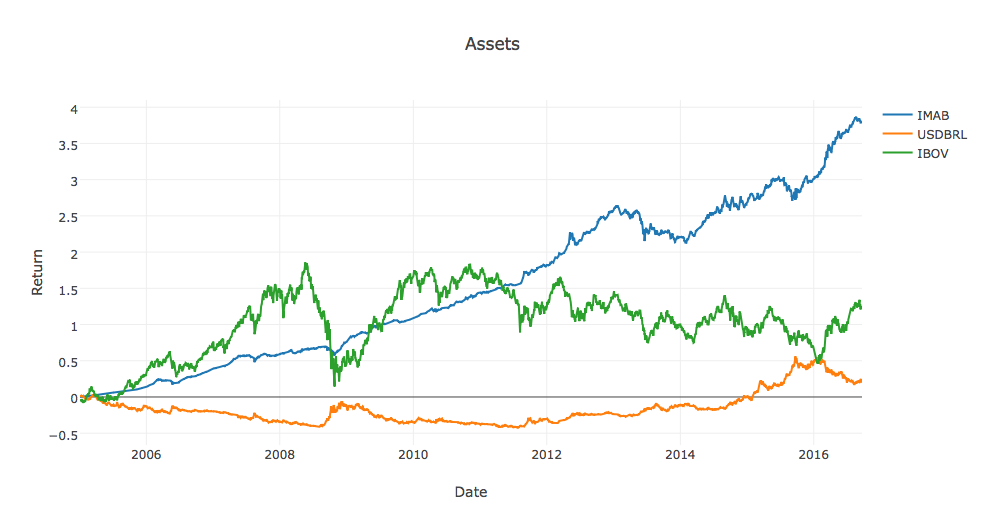
\includegraphics[width=\linewidth]{Assets.png}
  \caption{Assets Daily Return}
  \label{fig:Assets}
\end{figure}

\section{Methodology}

Our sample was comprised of daily returns ranging from 2005 to September 2016.

We first located all the rebalancing dates for the corresponding frequencies and afterwards, for each date, we recalculated the efficient frontier using all the previous data. With that frontier we could calculate the new weights. The frontiers are calculated with a non shorting restriction.

Then we computed returns for the 9 portfolios (3 strategies in 3 frequencies each), ignoring transaction costs.

To draw our conclusions we first compared all the frequencies within each strategy and then all the strategies within each frequency.

\section{Results}

\subsection{Across Frequencies}

Our goal is to find which frequency works best.

\subsubsection{Equally Weighted Strategy}

\begin{figure}[H]
  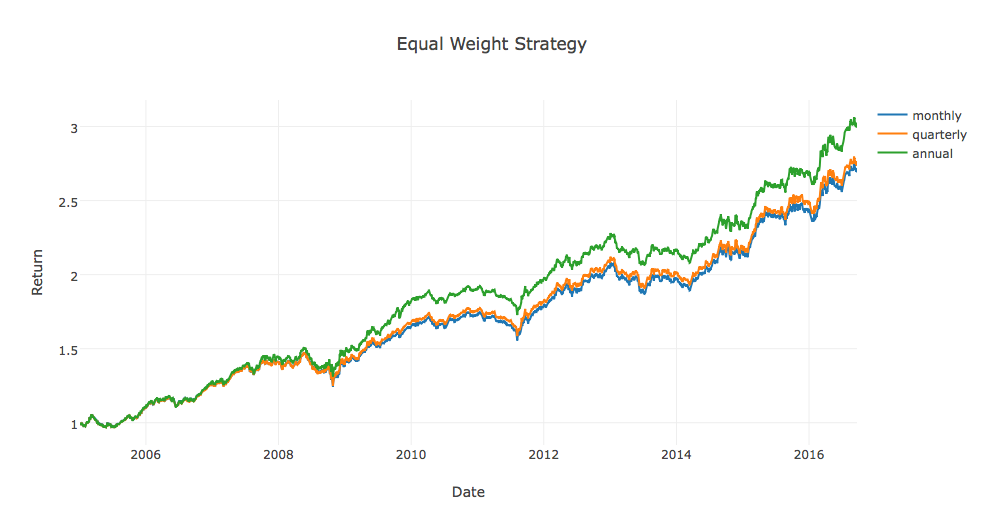
\includegraphics[width=\linewidth]{EWFrequencies.png}
  \caption{Equally Weighted Portfolios}
  \label{fig:EWFrequencies}
\end{figure}

In figure \ref{fig:EWFrequencies} we can see that the annual rebalance significantly outperforms the others, moreover the monthly rebalance has the worst performance. Indicating that the lower the frequency the better are the returns.

\subsubsection{Minimum Variance Strategy}

\begin{figure}[H]
  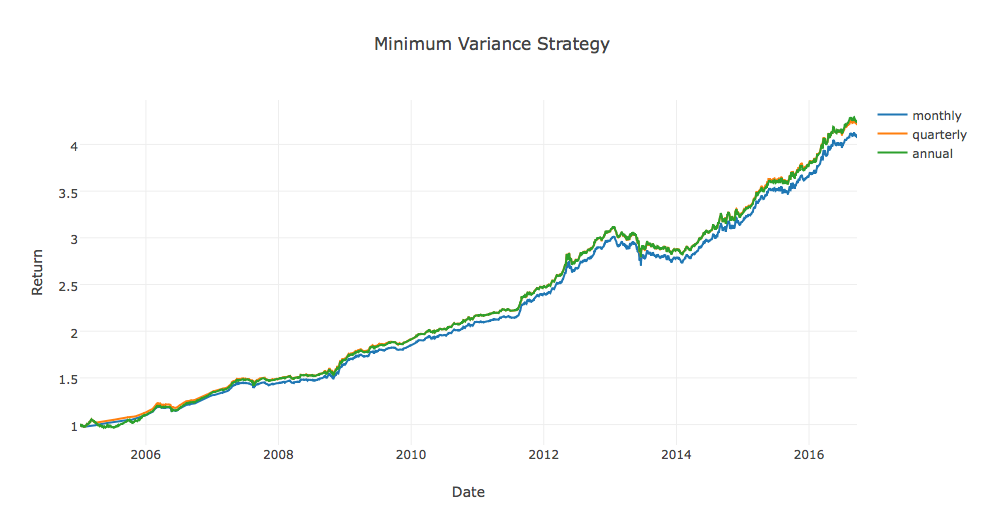
\includegraphics[width=\linewidth]{MVFrequencies.png}
  \caption{Minimum Variance Portfolios}
  \label{fig:MVFrequencies}
\end{figure}

In figure \ref{fig:MVFrequencies} we can again see that the annual rebalance significantly outperforms the others. Although it is not highly different from the quarterly rebalance. Indicating again that lower frequencies work best.

\subsubsection{Tangency Strategy}

\begin{figure}[H]
  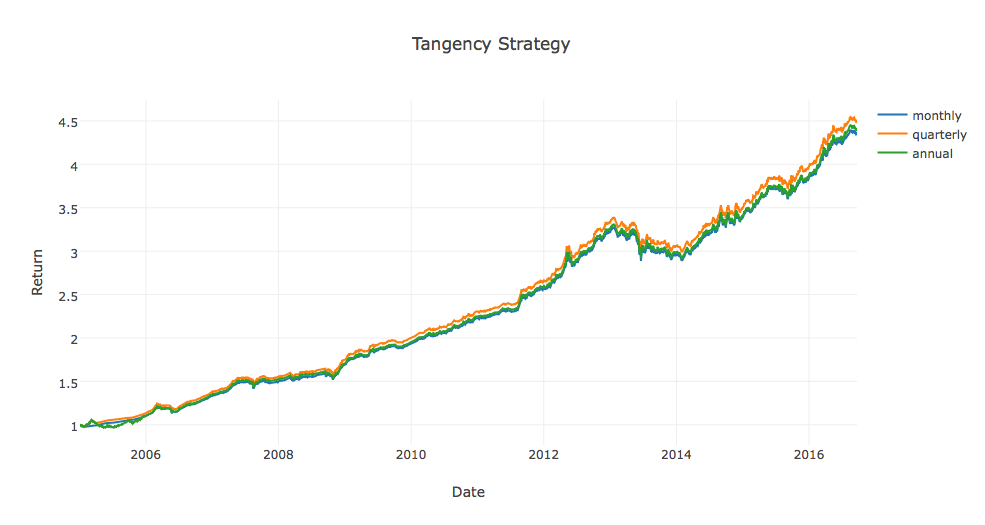
\includegraphics[width=\linewidth]{TGFrequencies.png}
  \caption{Tangency Portfolios}
  \label{fig:TGFrequencies}
\end{figure}

In figure \ref{fig:TGFrequencies} we find the same cardinal results we found for Equally Weighted Portfolios, with lower frequencies outperforming higher frequencies. Except that in this setup the quarterly frequency outperforms the annual.

\subsection{Across Strategies}

Our goal is to find which strategy works best.

\subsubsection{Monthly Frequency}

\begin{figure}[H]
  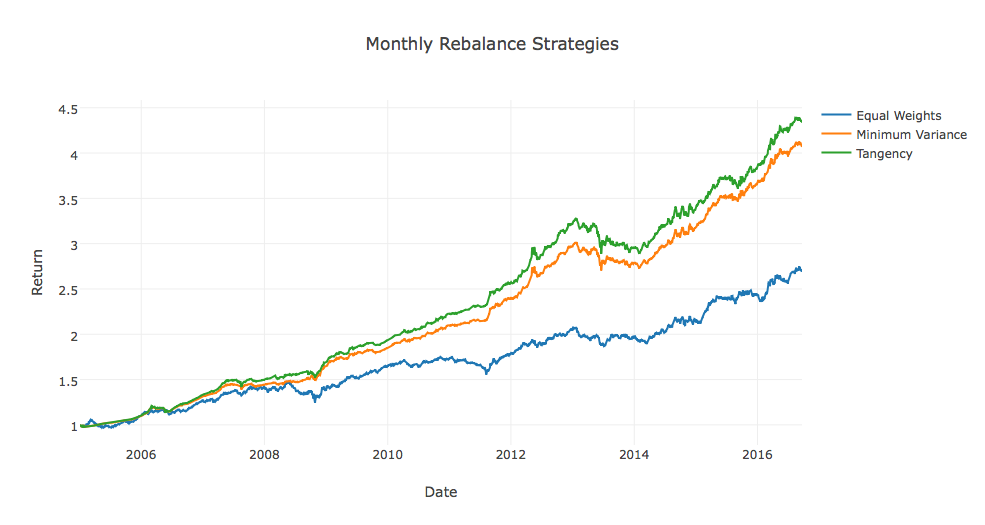
\includegraphics[width=\linewidth]{MStrat.png}
  \caption{Monthly Frequency}
  \label{fig:MStrat}
\end{figure}

For monthly rebalanced portfolios the Equally Weighted strategy vastly underperforms the others and the Tangency portfolio performs best.

\subsubsection{Quarterly Frequency}

\begin{figure}[H]
  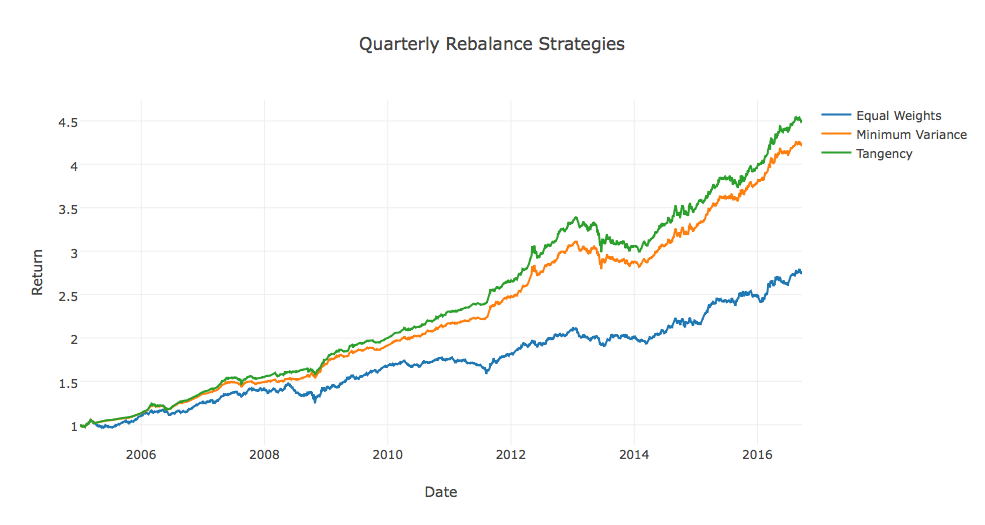
\includegraphics[width=\linewidth]{QStrat.png}
  \caption{Quarterly Frequency}
  \label{fig:QStrat}
\end{figure}

For quarterly rebalanced portfolios we find very similar results in which again the Equally Weighted strategy vastly underperforms the others and the Tangency portfolio performs best.

\subsubsection{Annual Frequency}

\begin{figure}[H]
  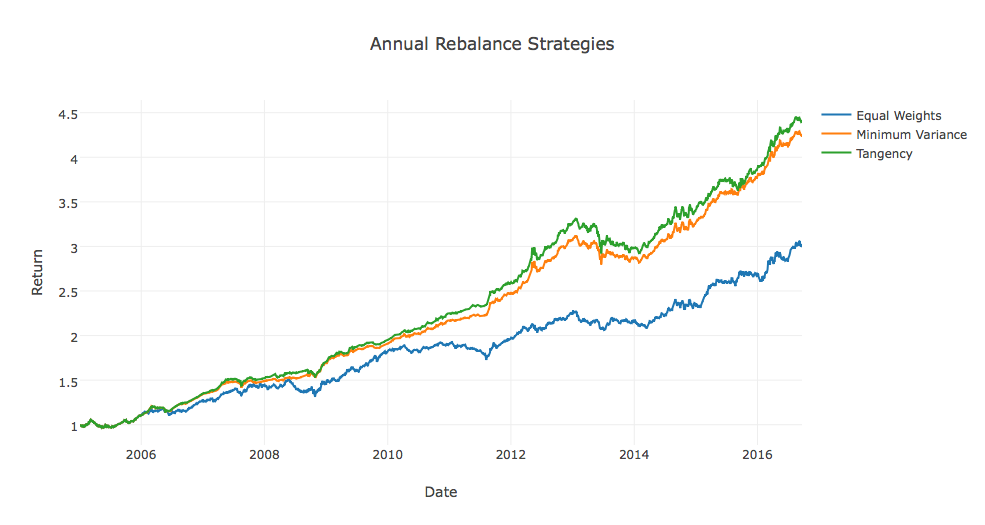
\includegraphics[width=\linewidth]{AStrat.png}
  \caption{Annual Frequency}
  \label{fig:AStrat}
\end{figure}

For annually rebalanced portfolios we find cardinally similar results in which again the Equally Weighted strategy vastly underperforms the others and the Tangency portfolio performs best.

\subsection{Monte Carlo Simulation}

After generating a 1000 random scenarios ,we ranked them according to equally weighted mean returns and picked the 1\% and 5\% worst scenarios to backtest the strategies.

The real and chosen scenarios are shown in figures \ref{fig:Real}, \ref{fig:5Var} and \ref{fig:1Var}.

\begin{figure}[H]
  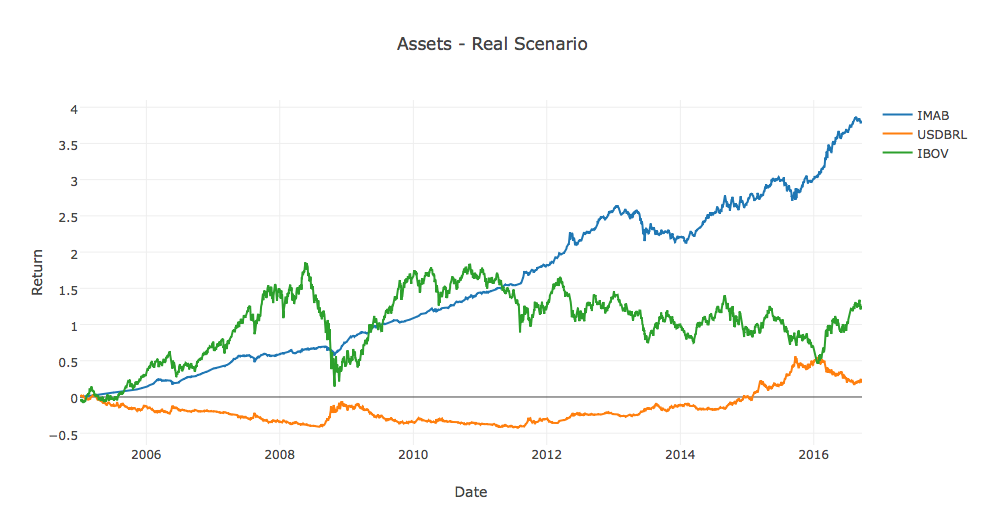
\includegraphics[width=\linewidth]{Real.png}
  \caption{Assets Real Performance}
  \label{fig:Real}
\end{figure}

\begin{figure}[H]
  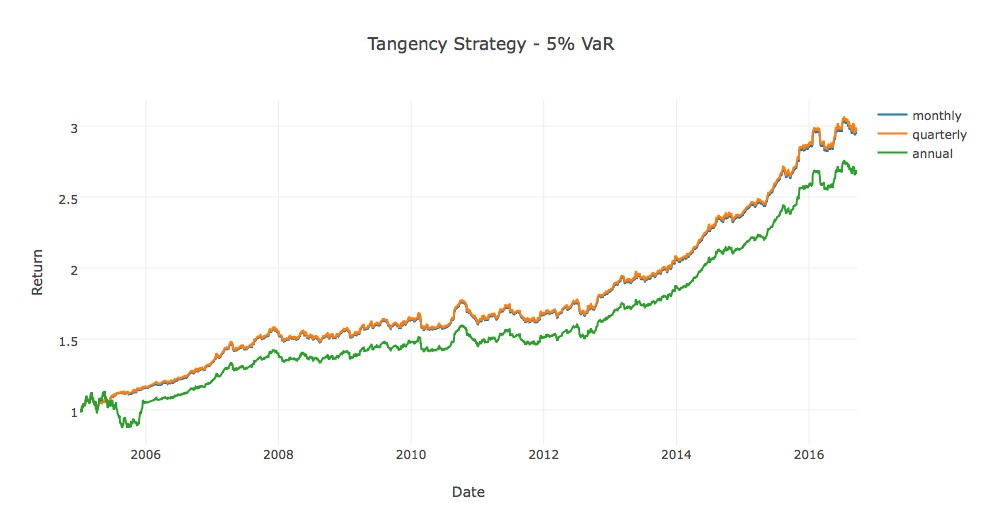
\includegraphics[width=\linewidth]{5Var.png}
  \caption{5\% Worst Scenario}
  \label{fig:5Var}
\end{figure}

\begin{figure}[H]
  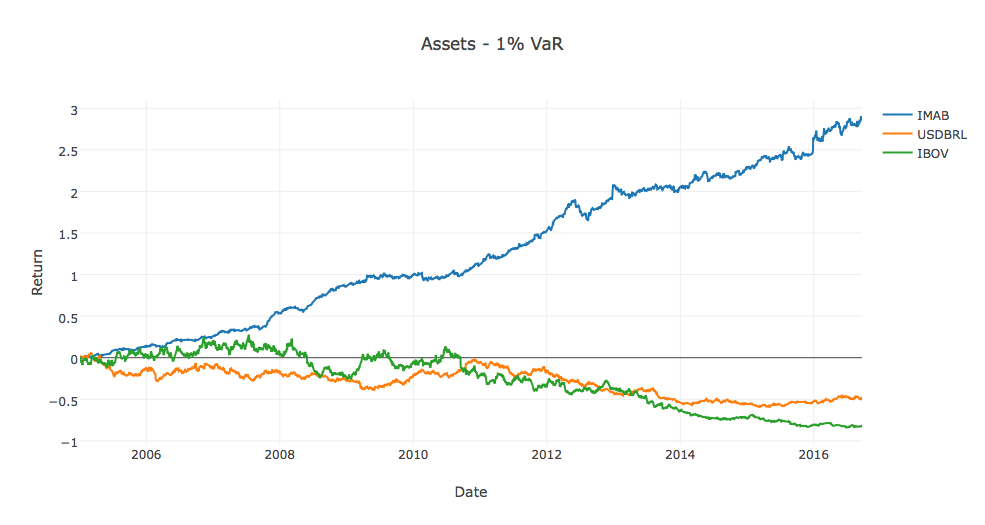
\includegraphics[width=\linewidth]{1Var.png}
  \caption{1\% Worst Scenario}
  \label{fig:1Var}
\end{figure}

\subsection{Across Frequencies}

Our goal is to find which frequency works best. For simplicity we will only look at Tangency Portfolios.

\subsubsection{5\% Worst}

\begin{figure}[H]
  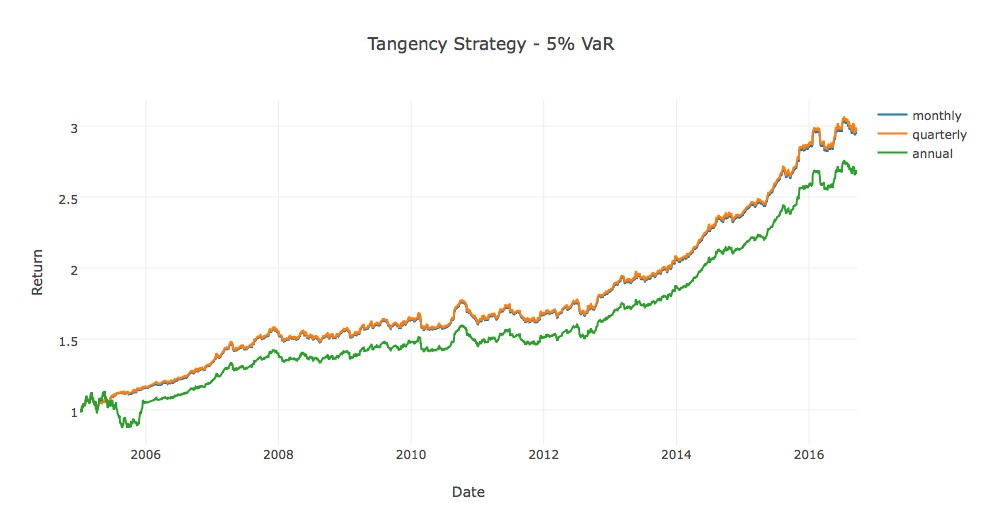
\includegraphics[width=\linewidth]{TG5.png}
  \caption{5\% Worst Scenario - Tangency Portfolios}
  \label{fig:TG5}
\end{figure}

In figure \ref{fig:TG5} we can see that annual rebalancing vastly underperforms the other frequencies, contradicting our previous findings.

\subsubsection{1\% Worst}

\begin{figure}[H]
  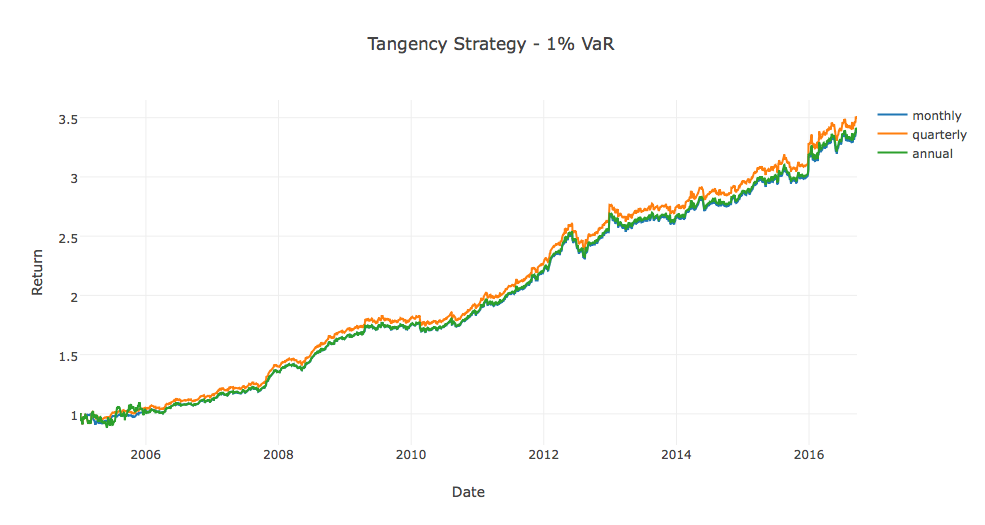
\includegraphics[width=\linewidth]{TG1.png}
  \caption{1\% Worst Scenario - Tangency Portfolios}
  \label{fig:TG1}
\end{figure}

In figure \ref{fig:TG1} we can see that annual rebalancing seems to underperform the other frequencies, also contradicting our previous findings. Although for this scenario the evidence is not as strong.

\subsection{Across Strategies}

Our goal is to find which strategy works best. For simplicity we will only look at Quarterly Frequency.

\subsubsection{5\% Worst}

\begin{figure}[H]
  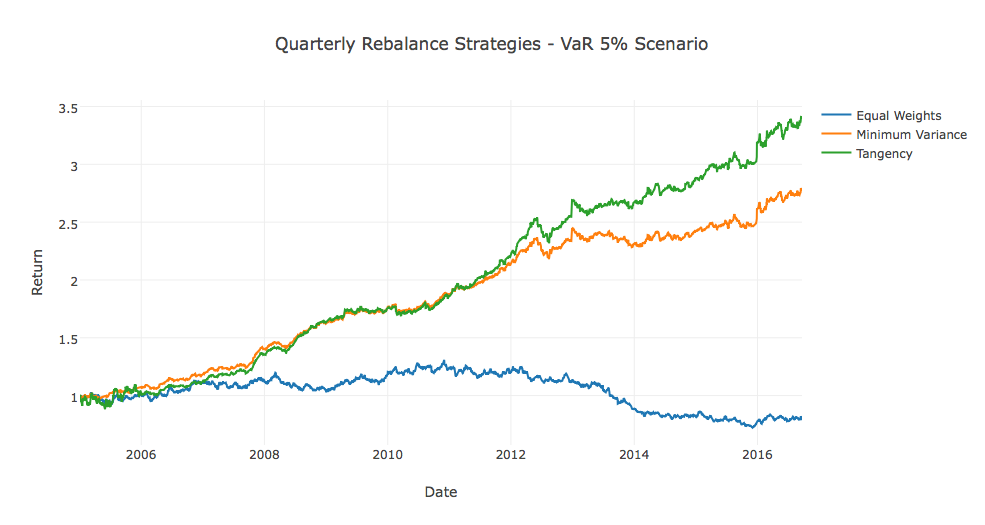
\includegraphics[width=\linewidth]{Q5.png}
  \caption{5\% Worst Scenario - Quarterly Rebalanced Portfolios}
  \label{fig:Q5}
\end{figure}

In figure \ref{fig:Q5} we find the same cardinal results as before, i.e., the Tangency portfolio outperforms the Minimum Variance portfolio which outperforms the Equally Weighted portfolio. Thus, indicating robustness of our findings.

\subsubsection{1\% Worst}

\begin{figure}[H]
  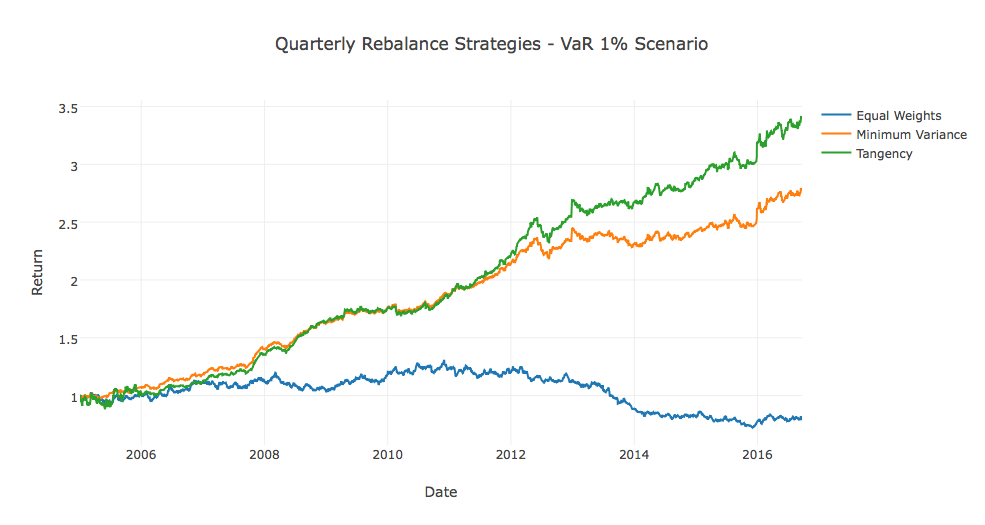
\includegraphics[width=\linewidth]{Q1.png}
  \caption{1\% Worst Scenario - Quarterly Rebalanced Portfolios}
  \label{fig:Q1}
\end{figure}

In figure \ref{fig:Q1} once more we find the same cardinal results as before. Again, indicating robustness of our findings.

\section{Conclusion}

In our initial Brazilian sample we first find evidence that lower frequencies are better than higher. That makes sense for a bullish market, in which frequent rebalances would prevent a long-only portfolio from pocketing its gains. The evidence is not strong though.

Secondly, for the same sample, we find more clear evidence that the Tangency strategy outperforms the others and that the Equally Weight strategy underperforms the others.

Since this could be considered a small sample, and also that the interest in rebalancing strategies is focused on preventing losses we decided to look at stress scenarios generated by Monte Carlo Simulation.

The two chosen Stress Scenarios bring evidence that our conclusion regarding frequency is not valid for bearish markets, which is consistent with the proposed explanation, and reinforces our conclusion regarding the strategies.



\end{document}